\section{PACXX}
\textit{PACXX} is a unified programming model that uses a custom compiler based on \textit{Clang} and \textit{LLVM}. It is a research project created by Michael Haidl and Sergei Gorlatch, both from University of Münster, Germany. The information in this section is based upon their \textit{PACXX} paper released in 2014\cite{pacxxPaper}. \textit{PACXX} is not officially released yet and there are no given release date, but the compiler can be found on \textit{Github}\cite{pacxxGithub}.

\subsection{Goals}
The \textit{PACXX} paper states that \textit{OpenCL} and \textit{CUDA} are error-prone since with these approaches, host code is written in \textit{C}/\textit{C++} with a restricted, \textit{C}-like API to handle memory management, and device specific code is written with a parallel programming model. The aim of \textit{PACXX} is to avoid the traditional pitfalls of GPU programming by unifying host and device code and thereby allowing a developer to utilize \textit{C++14} and \textit{STL} features.

\subsection{Programming Model}
As the goal of \textit{PACXX} suggests, the programming model is similar to a regular \textit{C++} approach, such that the developer will not have to change mindset when programming. There are some exceptions; The developer still needs to evaluate the threads and blocks she want to use. The developer must use the \texttt{kernel} class that \textit{PACXX} provides to construct a kernel function. Lastly, \textit{PACXX} generates and compiles device code at run-time, and there are no restrictions as to what a kernel function can call, but all code used in combination with a kernel must be known at run-time. Another restriction is that functions from pre-compiled libraries cannot be used by a kernel function.

Listing \ref{code:saxpyPACXX} shows a \textit{SAXPY} implementation using \textit{PACXX}. A lambda function called \texttt{saxpy} is created on line \ref{code:saxpyPACXX:lambda}, which describes \textit{SAXPY}. The thread id will be fetched, as seen on line \ref{code:saxpyPACXX:fetchID}, and then the elements corresponding to that thread of each vector will be used for the \textit{SAXPY} computation. The amount of threads and blocks are determined at line \ref{code:saxpyPACXX:threads} and \ref{code:saxpyPACXX:blocks}. Then, at line \ref{code:saxpyPACXX:kernel}, the kernel function is constructed using the \textit{PACXX} provided \texttt{kernel} class. The \textit{SAXPY} computation is executed at line \ref{code:saxpyPACXX:exec}.

\begin{lstlisting}[caption={\textit{SAXPY} computation in \textit{PACXX}.}, label={code:saxpyPACXX}]
main() {
  size_t = 1 << 24;
  float a = 2;
  std::vector<float> x(n), y(n), z(n);

  auto saxpy = [](const float& a, const vector<float>& x, const vecotr<int>& y, vector<float>& z) { ~\label{code:saxpyPACXX:lambda}~
    auto i = Thread::get().global.x; ~\label{code:saxpyPACXX:fetchID}~
    if (i >= x.size()) return;
    z[i] = x[i] * a + y[i];
  };

  size_t threads = 128; ~\label{code:saxpyPACXX:threads}~
  size_t blocks = (n + (threads * 2 - 1)) / (threads * 2); ~\label{code:saxpyPACXX:blocks}~

  auto saxpy_gpu = kernel(saxpy, {{blocks}, {threads}}); ~\label{code:saxpyPACXX:kernel}~
  saxpy_gpu(a, x, y, z); ~\label{code:saxpyPACXX:exec}~
}
\end{lstlisting}

\subsection{Implementation}
\textit{PACXX} is a framework centered around a compiler created with \textit{LLVM}, named \textit{pacxx++}. Using a special purpose compiler allows for quality of life features, such as defining kernel functionality in \textit{C++11} lambdas, at the cost of forcing that compiler to be used by the developer. The compilation is multi-staged, meaning that the main program is statically compiled, and the kernels are compiled before use, allowing kernels to vary depending on run-time state.

An important feature of \textit{PACXX} is that the code written by the developer is standard \textit{C++}, and can be compiled and executed on many platforms. The \textit{pacxx++} compiler is able to identify lambdas that can be compiled for a GPU, and create a unified programming experience.

On figure \ref{fig:pacxxCompilation} it is shown how a program compiled with \textit{pacxx++} includes the \textit{PACXX Run-time}. This run-time is able to generate \textit{LLVM Intermediate Representation} code and translate that to either \textit{PTX} code for the \textit{CUDA Run-time} or \textit{SPIR} code for the \textit{OpenCL Run-time}, using the \textit{LLVM} support for those targets.
\begin{figure}[H]
\center
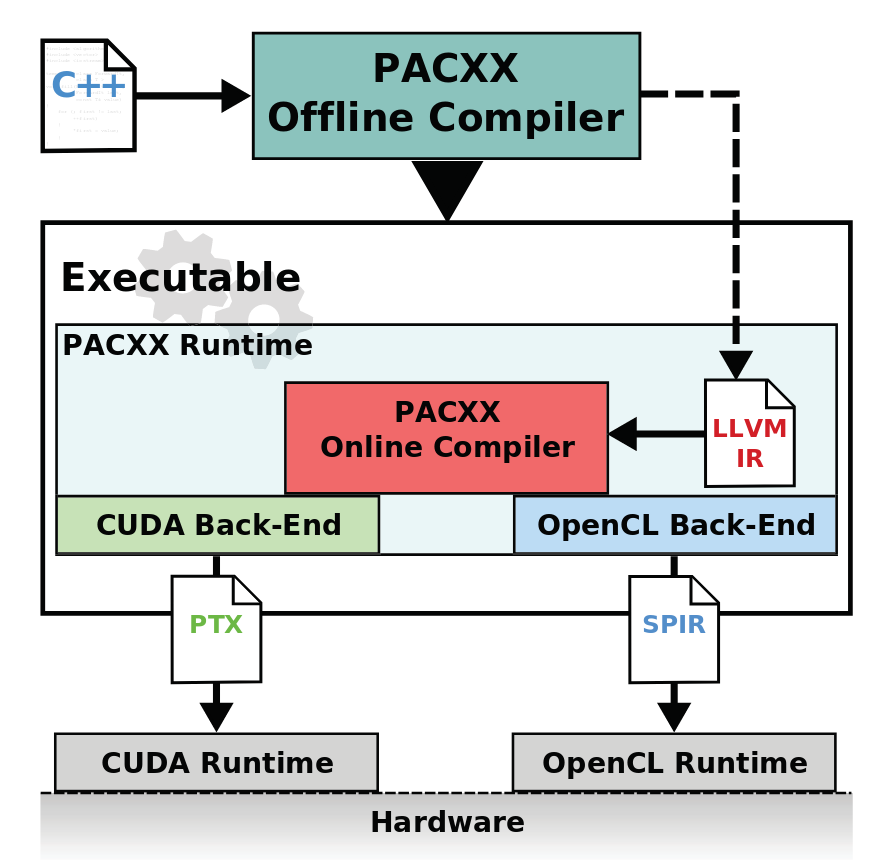
\includegraphics[width=0.8\textwidth]{chapters/relatedWorks/figures/pacxx_compilation_cool.png}
\caption{PACXX Compilation Process\cite{pacxxPaper2}.}
\label{fig:pacxxCompilation}
\end{figure}

\subsection{Key Points}
\textit{PACXX} allows a developer to write device specific code with \textit{C++14} lambdas with few restrictions, and must still take threads and blocks into account. 

\textit{PACXX} uses \textit{LLVM} to generate \textit{PTX} and \textit{SPIR} code at run-time. This is interesting as it provides more opportunities and freedom for abstractions than a static header library would. \textit{PACXX} is also multi-staged such that run-time compiled kernels can vary depending on state.
